\chapter[面向车载信息物理融合的超视距碰撞预警原型系统设计及实现]{面向车载信息物理融合的超视距碰撞预警原型系统\\设计及实现}
本章将针对基于车载信息物理融合的超视距碰撞预警原型系统设计与实现进行研究。
内容安排如下:
\ref{section 5-1} 节是本章的引言,介绍车联网碰撞预警系统研究现状和目前研究的不足以及本章的主要贡献。
\ref{section 5-2} 节介绍超视距碰撞预警场景。
\ref{section 5-3} 节设计了基于视图修正的碰撞预警算法。
\ref{section 5-4} 节在基于真实车辆轨迹的仿真场景中对所提算法进行了性能验证。
\ref{section 5-5} 节搭建了硬件在环,并在真实车联网环境中对所提算法进行了有效性验证。
\ref{section 5-6} 节总结本章的研究工作。

\section{引言}\label{section 5-1}

车辆碰撞预警系统作为 ITS 的典型安全应用,已得到学术界与工业界的广泛关注。
现有大多数车辆碰撞预警系统都基于超声波雷达或激光雷达等测距传感器进行实现\cite{song2018real, wu2019series},并取得了不错的效果,但是这些方案都存在非视距的问题。
随着近年来计算机视觉的发展,部分研究尝试利用车载摄像头的实时视频流来进行车辆碰撞检测 \cite{wang2016vision, song2018lane}。
然而,基于计算机视觉的方法需要大量数据传输和密集计算,这对系统性能提出了更高的要求,在实际部署中无法保证系统的实时响应。 
部分研究基于车联网通信实现碰撞预警\cite{hafner2013cooperative, gelbal2017elastic}。
但是,无线通信中传输时延和数据包丢失等问题是不可避免的,而车辆碰撞预警系统对实时性具有非常严苛的要求,这使得在车联网中实现实时可靠的安全关键型服务变得更加困难。
因此,面向真实复杂性车联网通信环境,如何有效获得实时准确的边缘视图,在此基础上,提供高质量的碰撞预警服务是具有挑战性与实用价值的。

基于以上分析,本章致力于设计及实现真实复杂性车联网环境中超视距碰撞预警原型系统。
本章的主要贡献总结如下:
第一,提出了基于视图修正的碰撞预警(View-Calibration-based Collision Warning, VCCW)算法,其通过结合通信时延估计和丢包检测来修正视图,从而提高碰撞预警系统的及时性和准确性。
具体地,基于真实车联网环境开展了现场测试并得到了 V2I 通信应用层时延数据,在此基础上,对车联网V2I通信的传输时延进行拟合,推导出了基于稳定分布的传输时延拟合模型。
另一方面,根据车辆位置和数据传输频率的历史信息,设计了一个丢包检测机制。
第二,基于真实车辆轨迹建立了仿真实验模型。
具体地,在德国科隆市选取具有不同特征(如交通密度、车辆速度、车辆加速度)的交叉路口并导入真实世界的车辆轨迹。
实现了所提算法与两种传统算法,其中包括基于云的碰撞预警(Cloud-Based Collision Warning, CCW)和基于边缘的碰撞预警(Edge-Based Collision Warning, ECW)。
CCW 和 ECW 均未考虑对视图进行修正。
仿真实验结果表明,与传统方法相比,VCCW 在碰撞预警的查全率和查准率方面都具有优势。
第三,基于 C-V2X 通信设备,搭建了硬件在环试验平台,并分析了不同数据包大小对 C-V2X 端到端传输时延的影响。
进一步,在真实车联网环境中,实现了基于车载信息物理融合的超视距碰撞预警原型系统,验证了本系统的可行性与有效性。


\section{超视距碰撞预警场景}\label{section 5-2}

本章将介绍超视距碰撞预警场景,如图 \ref{fig 5-1} 所示,具有短无线电覆盖范围的通信基础设施(如RSU、5G小基站)作为边缘节点,其在物理位置上更接近车辆并具有一定的计算能力。
同时,具有广泛覆盖范围的通信基础设施(如 5G 蜂窝网络基站)作为云节点。
车辆可通过 V2C 和 V2I 通信分别与云节点和路侧边缘节点进行通信。
虽然云节点拥有足够强大的算力来满足其覆盖范围内所有车辆的任务请求,但也会受到通信带宽的限制,如果当前云节点服务的车辆进行并发的数据传输,极大可能产生严重的带宽竞争,造成系统的吞吐量急剧下降。
与传统的基于云的服务相比,基于车载边缘计算的服务不仅减少了无线通信时延,而且通过将计算任务卸载到分布式的边缘节点上,提高了系统的响应性和可扩展性。
在本场景中,两辆汽车(即 $v_1$ 和 $v_2$)正从两个方向接近没有交通信号灯的十字路口。
在两车均不在对方视野的情况下,发生碰撞事故的概率大大增加。
为避免上述事故的发生,需要实现非视距场景下的车辆碰撞预警,因此,本章提出了基于逻辑视图的超视距碰撞预警系统。
车辆定期通过 V2I 通信将实时状态上传至边缘节点,包括全球定位系统(Global Positioning System, GPS)坐标、速度、加速度、方向等。
随后,边缘节点对覆盖范围内的车辆传感数据进行处理,构建出反映车辆实时状态的逻辑视图,以支持基于车辆轨迹预测的碰撞预警服务。
然而,车辆传感数据容易受到外界条件影响而出现偏差。
例如,由于卫星时钟偏差、大气时延和广播星历错误等原因,获得的 GPS 坐标可能出现偏移 \cite{liu2013improving}。
此外,数据包丢失也使边缘节点对移动车辆的实时位置估计变得更加困难。

\begin{figure}[h]
	\centering
	\includegraphics[width=0.9\columnwidth]{Fig5-1-example.pdf}
	\bicaption{超视距碰撞预警场景}{None-light-of-sight collision warning scenario}
	\label{fig 5-1}
\end{figure}

综上所述,尽管移动边缘计算新范式比传统的集中式云计算减少了通信时延,但由于不可避免且难以忽视的诸如传感器错误、传输时延和数据包丢失等问题,面向碰撞预警系统的边缘视图的有效构建仍然存在严峻的挑战。
图 \ref{fig 5-1} 显示了边缘节点构建的逻辑视图与真实交通视图的差异,其本质原因是边缘节点对车辆位置的不准确估计。
具体来说,假设车辆$v_1$在时间$t_1$的位置为$l_1$,且以$s_1 =$ 40 km/h 的速度接近十字路口。
同时,车辆$v_2$在时间$t_1$位于$l_3$并以$s_2=$ 25 km/h的速度接近同一路口。
车辆$v_1$和$v_2$在时间$t_1$同时向边缘节点发送实时状态。
然而,包含车辆$v_2$状态的数据包在V2I通信中丢失。
边缘节点在时间$t_2$接收到车辆状态信息,并形成车辆位置分布的逻辑视图,如图\ref{fig 5-1}所示。
假设数据大小为 500 kB,这对于典型的ITS应用来说是足够的\cite{liu2013improving}。
典型的车联网通信技术DSRC支持3$\sim$27 Mb/s的传输速率,其中3 Mb/s 被推荐用于传输安全关键信息\cite{kenney2011dedicated}。
因此,车辆状态的上传时间约为500 * 8 kb / 3 $\approx$ 1.3 s,即${t_2} - {t_1} \approx 1.3$ s。
在逻辑视图中,车辆$v_1$位于$l_1$,而$v_2$不存在。
然而如真实交通视图所示,车辆$v_1$和$v_2$的真实位置分别为$l_2$和$l_4$。
车辆$v_1$在逻辑车辆视图和真实交通视图之间的位置误差约为40 * 1000 / 3600 m/s * 1.3 $\approx$ 14 m,换言之,$d \approx$ 14 m。
从上述例子可以看出,如何在车联网中实现信息物理融合即构建一个实时准确的视图以支持不同的智能交通系统应用是迫切需要解决且极具挑战的问题。

\section{基于视图修正的碰撞预警算法}\label{section 5-3}

本章节提出了基于视图修正的碰撞预警算法,其通过拟合传输时延和检测丢包来修正边缘节点构建的逻辑视图,以提高碰撞预警的服务质量。
首先,基于真实车联网环境测试数据对V2I应用层传输时延进行拟合,得到基于稳定分布的V2I时延模型。
其次,基于数据传输频率和车辆位置的历史信息,设计了丢包检测机制。
最后,阐述了基于视图修正的碰撞预警算法的详细工作流程。

\subsection{应用层V2I时延拟合模型}

\begin{figure}[h]
\centering
  \includegraphics[width=0.8\columnwidth]{Fig5-2-delay.pdf}
  \bicaption[不同系统架构下的传输时延]{不同系统架构下的传输时延,云计算和车载边缘计算中数据包传输的平均时延分别为120${ms}$和77${ms}$}[Transmission delay under different system architectures]{Transmission delay under different system architectures where average delay of packets transmission in cloud and fog computing is 120 ms and 77 ms, respectively}
  \label{fig 5-2}
\end{figure}

本章根据真实车联网环境的现场测试数据分析了V2I通信的应用层传输时延。
在现场测试中,配备OBU的车辆通过V2I通信与RSU通信。
RSU作为边缘节点被安装在十字路口,与之相连的笔记本电脑充当RSU的计算单元。
当车辆接近十字路口时,通过V2I通信定期发送车辆状态,包括GPS坐标、速度、加速度、方向和时间戳。
边缘节点接收车辆数据包并计算V2I通信的应用层传输时延。
接下来,本章对真实车联网通信环境中的V2I传输时延进行建模。
具体地,根据对传输时延测试结果的观察,发现V2I通信的应用层传输时延分布并不服从高斯分布,而稳定分布是一种成熟的模型,适用于对非高斯过程进行估计。
本章节末尾的拟合结果表明,稳定分布可以相当准确地描述传输时延的特征和性质。
因此,本章利用稳定分布来拟合应用层V2I通信时延,其可以用如下的特征函数\cite{samoradnitsky2017stable}来描述
\begin{numcases}{E \exp (i t X)=}
\exp \left\{-\sigma^{\alpha}|t|^{\alpha}[1-i \beta \tan (\alpha \pi / 2) \operatorname{sgn}(t)]+i \mu t\right\}, &$\alpha \neq 1$ \notag \\
\exp \{-\sigma|t[1+i \beta(2 / \pi) \operatorname{sgn}(t) \ln (|t|)]+i \mu t\},  &$\alpha=1$
\end{numcases}
\noindent
其中 $X$ 是一个随机变量并服从稳定分布 $X \sim {S(\alpha, \beta, \mu, \sigma)}$, 且
\begin{numcases}{}
	\alpha \in \left( 0, 2\right] \notag \\
	\beta \in \left[ -1, 1 \right] \notag \\
	\mu \in \mathbb{R} \notag \\
	\sigma \in \mathbb{R}^{+}
\end{numcases}
其中$\alpha$是稳定性指数,当$\alpha=2$时,该稳定分布是高斯分布。
$\beta$是一个偏度参数,当$\beta=0$时,该稳定分布具有中心对称性,其对称中心为$\mu$。
$\alpha \neq 1$,$\beta > 0$和$\beta < 0$的情况分别对应于左偏度和右偏度。
$\sigma$是一个类似于方差的尺度参数。
特征函数$\phi(t)=E \exp (i t X)$完全决定了随机变量$X$概率分布的行为和特性,其中$t$为实数,$i$为虚数单位,$E$为期望值。
$\operatorname{sgn}(t)$ 是一个符号函数,其定义为:
\begin{numcases}{\operatorname{sgn}(t)=}
		1, &$t>0$ \notag \\
		0, &$t=0$ \notag \\
		-1, &$t<0$ 
\end{numcases}

本章采用回归模型来估计稳定分布的四个参数。
首先,给定大小为$n$的观测数据随机样本,记为$x_1, x_2, \ldots, x_n$,那么特征函数$\hat{\phi}(t)$可定义为
\begin{align}
	\hat{\phi}(t)&\!=\!\frac{1}{n} \sum_{j=1}^{n} \exp \left(i t x_{j}\right) \notag \\
	&\!=\!\frac{1}{n} \sum_{j=1}^{n}\left[\cos \left(t x_{j}\right)+\sin \left(t x_{j}\right) i\right] \notag \\
	&\!=\!\frac{1}{n} \sum_{j=1}^{n} \cos \left(t x_{j}\right)+i \frac{1}{n} \sum_{j=1}^{n} \sin \left(t x_{j}\right)
\end{align}
当 $\alpha \neq 1$, 可以得到
\begin{align}
	\phi(t) 
	&\!=\!E \exp (i t X) \notag \\ 
	&\!=\!\exp \left\{-\sigma^{\alpha}|t|^{\alpha}[1\!-\!i \beta \tan (\alpha \pi / 2) \operatorname{sgn}(t)]+i \mu t\right\} \notag \\ 
	&\!=\!\exp \left\{-\sigma^{\alpha}|t|^{\alpha}\!+\!\left[\mu t\!+\!\sigma^{\alpha}|t|^{\alpha} \beta \tan (\alpha \pi / 2) \operatorname{sgn}(t)\right] i\right\} \notag \\  
	&\!=\!\exp \left(-\sigma^{\alpha}|t|^{\alpha}\right) \exp \left[\left(\mu t\!+\!\sigma^{\alpha}|t|^{\alpha} \beta \tan (\alpha \pi / 2) \operatorname{sgn}(t)\right] i\right\} \notag \\ 
	&\!=\!\exp \left(-\sigma^{\alpha}|t|^{\alpha}\right) \cos \left[\mu t\!+\!\sigma^{\alpha}|t|^{\alpha} \beta \tan (\alpha \pi / 2) \operatorname{sgn}(t)\right] \notag \\ 
	&\!+\!\exp \left(-\sigma^{\alpha}|t|^{\alpha}\right) \sin \left[\mu t\!+\!\sigma^{\alpha}|t|^{\alpha} \beta \tan (\alpha \pi / 2) \operatorname{sgn}(t)\right] i 
\label{equ 5-5}
\end{align}
假设分布围绕中心$0$对称(即$\beta = 0$,$\mu = 0$),容易得到
\begin{equation}
	-\ln |\phi(t)|^{2}=2 \sigma^{\alpha}|t|^{\alpha}
\end{equation}
进一步可得
\begin{align} 
	\ln \left(-\ln | \phi(t)^{2}\right)
	&= \ln \left(2 \sigma^{\alpha}|t|^{\alpha}\right) \notag \\ 
	&=\ln \left(2 \sigma^{\alpha}\right)+\alpha \ln (|t|) 
\end{align}


通过回归$y_{k}=\alpha \omega_{k}+b$来估计$\alpha$和$\sigma$,其中${b=\ln \left(2 \sigma^{\alpha}\right)}$和${\omega_{k}=\ln \left(\left|t_{k}\right|\right)}$。
记$f\left(t_{k}\right)=\ln \left(-\ln \left|\phi\left(t_{k}\right)\right|^{2}\right)$并使用线性回归最小化均方误差。
\begin{align}
\left(\alpha^{*}, b^{*}\right) &=\underset{(\alpha, b)}{\arg \min } \sum_{k=1}^{K}\left(f\left(t_{k}\right)-y_{k}\right)^{2} \notag \\ &=\underset{(\alpha, b)}{\arg \min } \sum_{k=1}^{K}\left[\ln \left(-\ln \left|\phi\left(t_{k}\right)\right|^{2}\right)-\left(\alpha \omega_{k}+b\right)\right]^{2}  
\end{align}
然后,用最小平方法得到估计值$\hat{\alpha}$和$\hat{\sigma}$,即
$E_{(\alpha, b)}=\sum_{k=1}^{K}\left(f\left(t_{k}\right)-y_{k}\right)^{2}$,其中估计参数可通过求解下式获得。
\begin{numcases}{}
	\frac{\partial E_{(\alpha, b)}}{\partial \alpha} =2 \left(\alpha \sum_{k=1}^{K} \omega_{k}^{2}-\sum_{k=1}^{K}\left(f\left(t_{k}\right)-b\right) \omega_{k}\right) =0 \notag \\
	\frac{\partial E_{(\alpha, b)}}{\partial b} =2\left(K b-\sum_{k=1}^{K}\left(f\left(t_{k}\right)-\alpha \omega_{k}\right)\right) =0 
\end{numcases}
因此,估计值 $\hat{\alpha}$ 和 $\hat{\sigma}$ 可以表示为
\begin{numcases}{}
	\hat{\alpha}={ \sum_{k=1}^{K} f\left(t_{k}\right)\left(\omega_{k}-\bar{\omega}\right)}/{\sum_{k=1}^{K} \omega_{k}^{2}-\frac{1}{K}\left(\sum_{k=1}^{K} \omega_{k}\right)^{2}} \notag \\
	\hat{\sigma}=\sqrt[\hat{\alpha}]{ (\exp \hat{b}) / 2}
\label{equ 5-10}
\end{numcases}
其中
${\hat{b}=\frac{1}{K} \sum_{k=1}^{K}\left(f\left(t_{k}\right)-\hat{\alpha} \omega_{k}\right)}$
和 $\bar{\omega}=\frac{1}{K} \sum_{k=1}^{K} \omega_{k}$。


容易看出,$\phi(t)$的实部和虚部,即$\operatorname{Re} \phi(t)$和$\operatorname{Im} \phi(t)$,均可由公式\ref{equ 5-5}得到。
\begin{equation}
	\operatorname{Re} \phi(t)=\exp \left(-\sigma^{\alpha}|t|^{\alpha}\right) \cos \left[\mu t+\sigma^{\alpha}|t|^{\alpha} \beta \tan (\alpha \pi / 2) \operatorname{sgn}(t)\right]
\end{equation}
\begin{equation}
	\operatorname{Im} \phi(t)=\exp \left(-\sigma^{\alpha}|t|^{\alpha}\right) \sin \left[\mu t+\sigma^{\alpha}|t|^{\alpha} \beta \tan (\alpha \pi / 2) \operatorname{sgn}(t)\right]
\end{equation}
进一步,可得
\begin{equation}
	\arctan \left(\frac{\operatorname{Im} \phi(t)}{\operatorname{Re} \phi(t)}\right)=\mu t+\sigma^{\alpha}|t|^{\alpha} \beta \tan (\alpha \pi / 2) \operatorname{sgn}(t)
\end{equation}

由于估计量 $\hat{\alpha}$ 和 $\hat{\sigma}$ 是根据公式 \ref{equ 5-10}得到的, 因此可以通过回归$q_{l}=\mu+c d_{l}$并使 $\varphi\left(t_{l}\right)$与$q_{l}$之间的均方误差最小化来估计另外2个参数 $\beta$ 和 $\mu$, 其中 ${d_{l}=\operatorname{sgn}\left(t_{l}\right)\left|t_{l}\right|^{\alpha-1}}$、${c=\sigma^{\alpha} \beta \tan (\alpha \pi / 2)}$,以及$\varphi\left(t_{l}\right)=\frac{1}{t_{l}} \arctan \left(\frac{\operatorname{Im} \phi\left(t_{l}\right)}{\operatorname{Re} \phi\left(t_{l}\right)}\right)$。
\begin{align}
\left(c^{*}, \mu^{*}\right) 
&=\underset{(c, \mu)}{\arg \min } \sum_{l=1}^{L}\left(\varphi\left(t_{l}\right)-q_{l}\right)^{2} \notag \\ 
&=\underset{(c, \mu)}{\arg \min } \sum_{l=1}^{L}\left(\frac{1}{t_{l}} \arctan \left(\frac{\operatorname{Im} \phi\left(t_{l}\right)}{\operatorname{Re} \phi\left(t_{l}\right)}\right)-\mu-c d_{l}\right)^{2}  
\end{align}
$E_{(c, \mu)}=\sum_{l=1}^{L}\left(\varphi\left(t_{l}\right)-q_{l}\right)^{2}$,则可以通过求解公式\ref{equ 5-15}来估计参数 $\beta$ 和 $\mu$。
\begin{numcases}{}
	\frac{\partial E_{(e, \mu)}}{\partial c}=2\left(c \sum_{l=1}^{L} d_{l}^{2}-\sum_{l=1}^{L}\left(\varphi\left(t_{l}\right)-\mu\right) d_{l}\right)&$=0$ \notag \\
	 \frac{\partial E_{(c, \mu)}}{\partial \mu}=2\left(L \mu-\sum_{l=1}^{L}\left(\varphi\left(t_{l}\right)-c d_{l}\right)\right)&$=0$
	 \label{equ 5-15}
\end{numcases}
因此,估计量 $\hat{\beta}$ 和 $\hat{\mu}$ 可表示如下:
\begin{numcases}{}
	\hat{\beta}= \frac{\hat{c}}{\hat{\sigma}^{\hat{\alpha}} \tan (\hat{\alpha} \pi / 2)} \notag \\
	\hat{\mu}= \frac{1}{L} \sum_{l=1}^{L}\left(\varphi\left(t_{l}\right)-\hat{c} d_{l}\right)
\label{equ 5-16}
\end{numcases}
其中 
\begin{equation}
\hat{c}=\frac{\sum_{l=1}^{L} \varphi\left(t_{l}\right)\left(d_{l}-\bar{d}\right)}{\sum_{l=1}^{L} d_{l}^{2}-\frac{1}{L}\left(\sum_{l=1}^{L} d_{l}\right)^{2}}
\end{equation}
$\bar{d}=\frac{1}{L} \sum_{l=1}^{L} d_{l}$。

\begin{figure}[h]
\centering
  \includegraphics[width=0.8\columnwidth]{Fig5-3-delay-fitting.pdf}
  \bicaption{V2I应用层传输时延的概率密度函数}{Probability density function of application-layer V2I transmission delay}
  \label{fig 5-3}
\end{figure}

综上所述,给定观测数据集$X^{(0)}$,通过公式\ref{equ 5-10} 和公式\ref{equ 5-16},可以求解稳定分布的四个参数。
首先,给定观察数据集为$X^{(0)}=(x_1^{(0)}, x_2^{(0)}, \ldots, x_n^{(0)})$,在第$p$次迭代中,通过公式\ref{equ 5-18}对数据进行标准化。
\begin{equation}
x_{j}^{(p)}=\left(x_{j}^{(p-1)}-\mu_{p-1}\right) / \sigma_{p-1}, p = 1,2,\ldots
\label{equ 5-18}
\end{equation}
其中${\sigma_{0}=\left(x_{.72}-x_{.28}\right) / 1.654}$,$\mu_{0}$为25\%的截尾平均数,$x_{j}$是样本四分位数 \cite{fama1971parameter}。
本章选择最佳的$t_{k}=\pi k / 25, k=1,2,\ldots,K^{(p)}$\cite{koutrouvelis1980regression}来估计公式\ref{equ 5-10}中的$\hat{\alpha}^{(p)}$和$\hat{\sigma}^{(p)}$。
\begin{equation}
	{\hat{\alpha}^{(p)}=\frac{ \sum_{k=1}^{K^{(p)}} f\left(t_{k}\right)\left(\omega_{k}-\bar{\omega}\right)}{\sum_{k=1}^{K^{(p)}} \omega_{k}^{2}-\frac{1}{K}\left(\sum_{k=1}^{K^{(p)}} \omega_{k}\right)^{2}} } 
\end{equation}
\begin{equation}
	{\hat{\sigma}^{(p)}=\sqrt[\hat{\alpha}^{(p)}]{ (\exp \hat{b}^{(p)}) / 2}}
\end{equation}
其中 $f\left(t_{k}\right) = \ln \left(-\ln \left|\frac{1}{n} \sum_{j=1}^{n} \exp \left(i t_{k} x_{j}^{(p)}\right)\right|^{2}\right)$。

根据上述估计参数得到公式\ref{equ 5-16}中的另外两个估计参数$\hat{\beta}^{(p)}$和$\hat{\mu}^{(p)}$如公式\ref{equ 5-21}和\ref{equ 5-22}所示,其最佳$L^{p}$点为$t_{l}=\pi l / 25, l=1,2,\ldots,L^{(p)}$ \cite{koutrouvelis1980regression}。
\begin{equation}
\hat{\beta}^{(p)}= \frac{\hat{c}^{(p)}}{\bar{\sigma}^{\bar{\alpha}} \tan (\bar{\alpha} \pi / 2)}
\label{equ 5-21}
\end{equation}
\begin{equation}
\hat{\mu}^{(p)}= \frac{1}{L^{(p)}} \sum_{l=1}^{L^{(p)}}\left(\varphi\left(t_{l}\right)-\hat{c}^{(p)} d_{l}\right)
\label{equ 5-22}
\end{equation}
其中 $\bar{\alpha} =  {\hat{\alpha}^{(p)}}$ , $\bar{\sigma} =  {\hat{\sigma}^{(p)}}$,
\begin{equation}
\varphi\left(t_{l}\right) = \frac{1}{t_{l}} \arctan \left(\frac{ \sum_{j=1}^{n} \sin \left(t_l x_{j}^{(p)}\right)}{\sum_{j=1}^{n} \cos \left(t_l x_{j}^{(p)}\right)}\right)
\end{equation}

现场测试的1804个数据包传输时延被用于估计稳定分布模型,经过有限的迭代,得到了满足要求的四个估计参数。
图\ref{fig 5-3}显示了应用层时延的概率密度函数(Probability Density Function, PDF)。
结果显示,应用层时延分布几乎是对称的($\alpha = 1.77395$),并围绕平均值($\mu = 72.7343$)。
因此,有95\%的置信度,平均值的真值位于$71.9384$和$73.5301$的区间内。
可以看出,所得到的分布具有左偏度($\beta = 1$)且与均值的离散程度较大($\sigma = 13.3685$)。

\subsection{数据包丢失检测机制}

本章提出了一种基于历史信息的数据包丢失检测机制,其中历史信息包括数据传输频率和车辆位置。
首先,根据车辆的上传频率,边缘节点获取需要更新状态的车辆ID集合。
对于上传车辆集合中的车辆,如果边缘节点没有收到其上传的数据包,则可能存在以下两种情况:
第一,该车辆不在V2I通信范围内,导致数据包无法成功传递。
第二,该车辆在V2I通信范围内,但数据包在传输过程中丢失。
为了辨别这两种情况,在所提出的丢包检测机制中,边缘节点会根据历史位置判断车辆是否在通信范围内,如果在通信范围内却未收到相应数据包,则边缘节点认为该数据包已丢失。

不失一般性,本章考虑碰撞预警系统由单个边缘节点和若干辆车组成。
值得注意的是,该设置可直接扩展到多个边缘节点的情况。
在此场景中,集合$\mathbf{T}=\{1, \ldots, t, \ldots, T\}$表示离散时间片。
车辆集合用$\mathbf{V}=\{1, \ldots, v, \ldots, V\}$表示。
在时间 $t$,车辆 $v$ 的位置、速度、加速度分别用 $l_{v}^{t}$、$s_{v}^{t}$,以及$a_{v}^{t}$ 表示。
边缘节点用$e$表示,其位置用 ${l}_{e}$ 表示,且V2I通信范围用 $g_e$ 表示。
在时间 $t$, 车辆 $v$ 与边缘节点$e$之间的距离用 $\operatorname{dis}_{v, e}^{t}$ 表示。
如果 $\operatorname{dis}_{v, e}^{t} \leq g_e$,则车辆 ${v}$ 可以与边缘节点进行V2I通信。
在时间 $t$,边缘节点接收到若干个数据包,该数据包集合用 $\mathbf{M}_{t}=\{1, \ldots, m, \ldots, {M}_t\}$ 表示,其中 $m =(l_{v}^{t}, s_{v}^{t}, a_{v}^{t})$,$m \in \mathbf{M}_{t}$。
同时,边缘节点记录每个时间片接收到的数据包,即使用集合 ${\mathbf{H}_{t}} = \{\mathbf{M}_{t-{H}_{t}}, \ldots, \mathbf{M}_{t-2}, \mathbf{M}_{t-1}\}$ 来表示在时间 $t$的 历史记录,其中${H}_{t}$为历史记录信息的长度。
基于上述定义,本章所提的基于历史信息的数据包丢失检测机制分为以下两个步骤:

\textbf{1)记录:}
边缘节点维护车辆ID集合$\mathbf{ID}_{t}$以记录时间 $t$ 时V2I 通信覆盖范围内所有车辆。
$\mathbf{ID}_{t}$ 可通过上一时刻的值$\mathbf{ID}_{t-1}$进行初始化。 
当边缘节点在时间 $t$ 收到若干个数据包 $\mathbf{M}_{t}$ 时,对于 $m =(l_{v}^{t}, s_{v}^{t}, a_{v}^{t})$,${m} \in M_{t}$,如果边缘节点第一次收到车辆 $v$ 的数据包,即${v} \notin \mathbf{ID}_{t}$,则将 $v$ 加入 $\mathbf{ID}_{t}$,即$\mathbf{ID}_{t} = \mathbf{ID}_{t} \cup \{v\}$。
边缘节点搜索 $\mathbf{M}_{t}$ 并将所有车辆ID添加到集合 $\mathbf{ID}_{\mathbf{M}_{t}}$。

\textbf{2)检测:}
对于车辆 ${v} \in \mathbf{ID}_{t} \cup \mathbf{ID}_{\mathbf{M}_{t}}$,存在两种可能性:
(a)${v} \in \mathbf{ID}_{t} \setminus \mathbf{ID}_{\mathbf{M}_{t}}$,即车辆 $v$ 可以与边缘节点通信,但是边缘节点未收到它的数据包;
(b)${v} \in \mathbf{ID}_{t} \cap \mathbf{ID}_{\mathbf{M}_{t}}$,即车辆 $v$ 可以与边缘节点通信,并且边缘节点收到了它的数据包。
因此,对于(a),边缘节点搜索 ${\mathbf{H}_{t}}$ 获取车辆的最新位置 $l_v^t$。
边缘节点使用距离阈值 $\tau$ 和时间阈值 $\gamma$ 来检测车辆是否超出通信范围。
如果车辆 $v$ 与边缘节点$e$之间的距离 $\operatorname{dis}_{v, e}^{t} \geq g_e - \tau$,那么表示车辆 $v$ 正在离开通信范围,边缘节点将 $v$ 从 $\mathbf{ID}_{t}$ 中移除,即$\mathbf{ID}_{t}=\mathbf{ID}_{t} \setminus \{v\}$。
如果 $\operatorname{dis}_{v, e}^{t} < g_e - \tau$,则表示车辆 $v$ 可以与边缘节点通信,但是边缘节点未收到它的数据包。
预估的数据包接收时间为 $t_r$,如果 $t - t_r > \gamma$,则边缘节点认为数据包已丢失。
否则存在以下两种情况:车辆 $v$ 尚未发送数据包,或由于无线通信时延导致数据包暂未收到。

\subsection{工作流程}

本章节介绍基于视图修正的碰撞预警算法的具体流程,如算法5.1所示。
首先,基于V2I传输时延拟合模型估计数据包传输时延,并根据车辆速度和加速度更新其实时状态。
其次,检测丢失的数据包,并使用边缘节点中的历史记录更新它们的状态。
再次,使用模拟的传输时延来校准车辆轨迹以获得更加准确实时的逻辑视图。
进一步,基于修正的视图预测所有车辆未来的轨迹。
最后,通过计算每对车辆的车头时距并通过车头时距阈值来检测潜在碰撞。
VCCW具体步骤如下:

\SetKwInOut{KwIn}{输入}
\SetKwInOut{KwOut}{输出}

\begin{algorithm}[h]\small
\renewcommand{\algorithmcfname}{算法}
	\caption{基于视图修正的碰撞预警}
	\KwIn{车辆ID集合$\mathbf{ID}_{t}$、收到的数据包$\mathbf{M}_{t}$、历史记录${\mathbf{H}_{t}}$、车辆轨迹预测时间 $t_{\operatorname{pre}}$、碰撞预警距离阈值$\operatorname{dis}_{\operatorname{col}}$、车头时距阈值$\imath$}
	\KwOut{碰撞预警信息 $w_{v}^{t}$}
	初始化ID集合,$\mathbf{ID}_{t} = \mathbf{ID}_{t-1}$, $\mathbf{ID}_{\mathbf{M}_{t}} = \emptyset $ \\
	\For{$m \in \mathbf{M}_{t}$}{
		$\mathbf{ID}_{\mathbf{M}_{t}} =\mathbf{ID}_{\mathbf{M}_{t}} \cup \{v\}$\\
		\If{$v \notin \mathbf{ID}_{t}$}{
			$\mathbf{ID}_{t} = \mathbf{ID}_{t} \cup \{v\}$\\
		}
	}
	\For{$v \in \mathbf{ID}_{t} \cup \mathbf{ID}_{\mathbf{M}_{t}}$}{
		\If{$v \in \mathbf{ID}_{t} \setminus \mathbf{ID}_{\mathbf{M}_{t}}$}{
			搜索历史信息 ${\mathbf{H}_{t}}$ 并得到车辆最新数据包 $m$\\
			\If{$\operatorname{dis}_{v, e}^{t} \geq g_e - \tau$}{
				$\mathbf{ID}_{t} = \mathbf{ID}_{t} \setminus \{v\}$\\
			}
			\If{$\operatorname{dis}_{v, e}^{t} < g_e - \tau$ 且 $t - t_r > \gamma$}{
				$\mathbf{M}_{t} = \mathbf{M}_{t} \cup \{ m \}$\\
			}
		}
	}
	\For{$m \in \mathbf{M}_{t}$}{
		${t_{\operatorname{int}}} = t - {t_{r}} + t_{f}^v$,并通过公式\ref{equ 5-24}更新车辆位置\\
		\While{${t_{\operatorname{int}}} > t + t_{\operatorname{pre}}$}{
			$t = t + \frac{1}{\xi}$,并根据公式\ref{equ 5-24} 计算车辆位置 $l_v^{t}$ \\
			$\mathbf{Tra}_{v} = \mathbf{Tra}_{v} \cup \{ l_v^t \}$\\
		}
		$\mathbf{Tra} = \mathbf{Tra} \cup \{\mathbf{Tra}_{v}\}$
	}
	\For{$\mathbf{Tra}_{v} \in \mathbf{Tra}$ \songti{且} $\mathbf{Tra}_{v^{\prime}} \in \mathbf{Tra} \setminus \{ \mathbf{Tra}_{v}\}$}{
		\For{$l_v^t \in \mathbf{Tra}_{v}$ \songti{且} $l_{v^{\prime}}^{t^{\prime}} \in \mathbf{Tra}_{v^{\prime}}$}{
			\If{$\operatorname{dis}_{v, v^{\prime}}^{t, t^{\prime}} < \operatorname{dis}_{\operatorname{col}}$}{
				${h}_{v, v^{\prime}} = |t - t^{\prime}|$\\
				\If{${h}_{v, v^{\prime}} < \imath$}{
					$w_{v}^{t} = w_{v^{\prime}}^{t^{\prime}} = 1$\\
				}
			}
		}
	}
	\label{algorithm 5-1}
\end{algorithm}

\textbf{1)车辆ID集合更新:}
在时间 $t$ 初始化车辆ID集合 $\mathbf{ID}_{t}$ 和收到的数据包 $\mathbf{M}_{t}$ 的 ID集合 $\mathbf{ID}_{\mathbf{M}_{t}}$。
其中$\mathbf{ID}_{\mathbf{M}_{t}}$ 包含了接收数据包中的所有车辆ID。
如果车辆ID没有包含在 $\mathbf{ID}_{t}$ 中,则边缘节点将该车辆ID添加到 $\mathbf{ID}_{t}$ 中。

\textbf{2)数据包丢失检测:}
边缘节点通过数据包丢失检测机制得到数据包丢失的车辆集合,对于数据包丢失的车辆,边缘节点将在数据包历史记录${\mathbf{H}_{t}}$中搜索最新的车辆状态信息,并将其添加到$\mathbf{M}_{t}$中。

\textbf{3)基于车辆轨迹校准的视图修正:}
对于数据包$m \in \mathbf{M}_{t}$,边缘节点基于稳定分布生成符合V2I传输时延拟合模型的随机数来估计数据包的传输时延$t_{f}^v$。
在此基础上,边缘节点估计数据包的发送时间${\hat t_{c}} = {t_{r}} - t_{f}^v$。
时间$t$和数据包发送时间${\hat t_{c}}$之间的时间间隔为${t_{\operatorname{int}}} = t - {t_{r}} + t_{f}^v$。
进一步,边缘节点更新车辆$v$的位置信息。
\begin{numcases}{}
	{l_x}_v^t = {l_x}_v^{{\hat t_{c}}} + {t_{\operatorname{int}}} {s_x}_v^{{\hat t_{c}}} + \frac{{t_{\operatorname{int}}}^2 {a_x}_v^{{\hat t_{c}}}}{2} \notag \\
	{l_y}_v^t = {l_y}_v^{{\hat t_{c}}} + {t_{\operatorname{int}}} {s_y}_v^{{\hat t_{c}}} + \frac{{t_{\operatorname{int}}}^2 {a_y}_v^{{\hat t_{c}}}}{2}
\label{equ 5-24}
\end{numcases}
其中,${l_x}_v^{{\hat t_{c}}}$、${l_y}_v^{{\hat t_{c}}}$、${s_x}_v^{{\hat t_{c}}}$、${s_y}_v^{{\hat t_{c}}}$、${a_x}_v^{{\hat t_{c}}}$,以及${a_y}_v^{{\hat t_{c}}}$分别表示车辆$v$在X和Y坐标系中的位置、速度和加速度。

\textbf{4)车辆未来轨迹预测:}
对于车辆$v$,边缘节点在时间段$(t, t + t_{\operatorname{pre}})$内预测其未来轨迹,其中$t_{\operatorname{pre}}$是车辆轨迹预测时间。
边缘节点每隔$\frac{1}{\xi}$秒计算一次车辆位置,其中$\xi$为车辆位置更新频率,并将计算得到的新位置添加到车辆$v$的轨迹集合$\mathbf{Tra}_{v}$中。

\textbf{5)潜在碰撞检测:}
碰撞预警预警信息集合用 $\mathbf{W}_t = \{ 1, \ldots, w_{v}^{t}, \ldots, W_t\}$ 表示,其中 $w_{v}^{t}$ 是一个0-1变量,表示车辆$v$是否有潜在碰撞风险。
对于位置信息满足$l_v^t \in \mathbf{Tra}_{v}$ 且 $l_{v^{\prime}}^{t^{\prime}} \in \mathbf{Tra}_{v^{\prime}}$ 的车辆对,边缘节点计算两辆车的距离$\operatorname{dis}_{v, v^{\prime}}^{t, t^{\prime}}$。
如果$\operatorname{dis}_{v, v^{\prime}}^{t, t^{\prime}} < \operatorname{dis}_{\operatorname{col}}$,其中$\operatorname{dis}_{\operatorname{col}}$为碰撞预警距离阈值, 则假定车辆$v$和$v^{\prime}$经过同一点。
前车的车头通过道路上的某一点和后车的车头通过同一点之间的时间被定义为车头时距\cite{vogel2003comparison}。
因此,边缘节点计算两车间的车头时距 ${h}_{v, v^{\prime}} = |t - t^{\prime}|$,如果${h}_{v, v^{\prime}} < \imath$,其中$\imath$是车头时距阈值,碰撞预警信息将被触发,即$w_{v}^{t} = w_{v^{\prime}}^{t^{\prime}} = 1$。

\section{实验结果与分析}\label{section 5-4}

\subsection{实验设置}

首先,本章在仿真实验中使用了收集自德国科隆市约400平方公里区域约120万辆真实出租车轨迹的数据集\cite{uppoor2013generation}。
本章选取了5个具有不同交通特征的路口来进行碰撞预警仿真实验,不同场景的具体交通特征如表\ref{table 6-1}所示。
场景1、2和3中,实验开始时间分别为晚上10点、早上8点和晚上7点。
在场景4和5中,实验开始时间为下午4点和6点。
边缘节点安装在前三个场景的$(10422.0, 12465.3)$和最后两个场景的$(6097.1, 14870.0)$处。
每个实验的持续时间为100 s,V2I通信范围设置为500 m。

\begin{table}[h]\small
\centering
\bicaption{不同场景的交通特征}{Traffic characteristics of different scenarios}
\setlength{\tabcolsep}{9.5mm}{
\begin{tabular}{cccc}
\toprule
场景&车辆数量&平均速度 (km/h)&平均加速度 (m/s$^2$)\\
\midrule
1& 54& 50.44& 0.203\\
2& 81& 46.58& 0.007\\
3& 106& 38.1& 0.075\\
4& 85& 69.19& 0.165\\
5& 114& 69.05& 0.060\\
\bottomrule
\end{tabular}}
\label{table 6-1}
\end{table}

为了进一步比较所提算法的性能,本章实现了两种具有对比性的碰撞检测算法。
\begin{itemize}
	\item \textbf{基于云的碰撞预警}:其是在集中式的云计算架构中实现的。具体地,车辆将其状态信息上传到距离车辆较远的云服务器。在仿真实验中,使用现场测试实验获得的V2C传输时延来模拟车辆和云节点之间的通信时延。云服务器没有对视图进行修正,仅基于车辆状态预测潜在碰撞。
	\item \textbf{基于边缘的碰撞预警}:其实现在车载边缘计算架构中。具体地,车辆将其状态上传到附近的边缘服务器,并使用在真实世界场地测试中获得的V2I传输时延来模拟车辆和边缘服务器之间的通信时延。与基于云的碰撞预警类似,边缘节点在没有对视图进行修正的情况下预测潜在碰撞。
\end{itemize}

为了进一步评估所提算法的性能,本章首先定义以下指标:
预测的碰撞预警消息集合用$\mathbf{W}_{p}$表示,期望的碰撞预警集合用$\mathbf{W}_{d}$表示。
期望预警消息的数量$\left| \mathbf{W}_{d} \right|$是实验设置的预期碰撞数量,而预测的碰撞预警消息数量$\left| \mathbf{W}_{p} \right|$是碰撞预警系统预测的潜在碰撞数量。
此外,$\left| \mathbf{W}_{d} \cap \mathbf{W}_{p} \right|$表示预期的碰撞预警中实际成功预测的数量。
$\left| \mathbf{W}_{d} - \mathbf{W}_{p} \right|$是应该被触发但未被碰撞预警系统成功预测的预期预警数量,换句话说,它是$\mathbf{W}_{p}$中的预测失败的数量。
同样,$\left| {\mathbf{W}_{p} - \mathbf{W}_{d}} \right|$是错误预测的数量,即是碰撞预警系统预测的潜在碰撞,但不是预期的碰撞预警。
因此,定义查准率(Precision)和查全率(Recall)如下
\begin{equation}
	\operatorname{Precision} = \frac{{\left| {\mathbf{W}_{d} \cap \mathbf{W}_{p}} \right|}}{{\left| {\mathbf{W}_{d} \cap \mathbf{W}_{p}} \right| + \left| {\mathbf{W}_{p} - \mathbf{W}_{d}} \right|}}
\end{equation}
\begin{equation}
	\operatorname{Recall} = \frac{{\left| {\mathbf{W}_{d} \cap \mathbf{W}_{p}} \right|}}{{\left| {\mathbf{W}_{d} \cap \mathbf{W}_{p}} \right| + \left| {\mathbf{W}_{d} - \mathbf{W}_{p}} \right|}}
\end{equation}

\subsection{实验结果与分析}

\begin{figure}[h]
     \centering
     \subfloat[][]{\includegraphics[width=0.5\columnwidth]{Fig5-5a-different-scenarios.pdf}}
     \subfloat[][]{\includegraphics[width=0.5\columnwidth]{Fig5-5b-different-scenarios.pdf}}
     \bicaption[不同交通场景下的性能对比]{不同交通场景下的性能对比,其中不场景的交通特征列于表\ref{table 6-1}中。(a)查准率(b)查全率}[Performance comparison under different scenarios]{Performance comparison under different scenarios, the traffic characteristics of which are listed in Table. \ref{table 6-1}. (a) Precision (b) Recall}
     \label{fig 5-5}
\end{figure}

\textbf{1) 不同交通场景的影响:}
图 \ref{fig 5-5} 比较了三种算法在不同交通场景下的性能,其中选取了五个具有不同交通特征的场景。
图 \ref{fig 5-5}(a)比较了三种算法的查准率。
显然,VCCW 在所有场景下都取得了最高的查准率。
主要原因是得益于VCCW 中对于边缘视图的修正,车辆状态更接近实时状态,换句话说,基于修正视图的碰撞预警可以提供更加准确的服务。
以上也可在图\ref{fig 5-5}(b)中得以证明,其比较了三种算法的查全率。
显然,在所有交通场景下,基于修正视图的碰撞预警都可以提高查准率和查全率。

\textbf{2) 不同车头时距阈值的影响:}
图\ref{fig 5-6} 比较了三种算法在不同车头时距阈值下的性能,其中车头时距阈值从1s 增加至 5s。
车头时距是两辆车的车头通过一个点之间的时间间隔,因此,通过车头时距阈值来评估两车发生潜在碰撞的风险。
显然,如果车头时距阈值小,预测的碰撞预警消息数量也会随之减少。
可以观察到,随着车头时距阈值的增加,查准率随之升高,这是因为当车头时距阈值增加时,预测的碰撞预警消息数量也随之增加。
因此,预测成功在整体预测数量中的占比也随之增加,即查准率的提升。
同理,随着车头时距阈值的增加,查全率随之下降。
图\ref{fig 5-6}(a)比较了三种算法的查准率。
可以看到,VCCW 在不同车头时距阈值下都取得了最高的查准率。
图\ref{fig 5-6}(b)比较了三种算法的查全率。
值得注意的是,ECW的性能明显高于CCW,这是因为基于边缘的碰撞预警可以利用分布式车载边缘计算架构带来的更低的数据包传输时延,使得边缘构建的视图与云端构建的视图相比更加实时。

\begin{figure}[h]
     \centering
     \subfloat[][]{\includegraphics[width=0.5\columnwidth]{Fig5-6a-different-headways.pdf}}
     \subfloat[][]{\includegraphics[width=0.5\columnwidth]{Fig5-6b-different-headways.pdf}}
     \bicaption[不同车头时距阈值下的性能对比]{不同车头时距阈值下的性能对比,其中车头时距阈值从1s 增加至 5s。(a)查准率(b)查全率}[Performance comparison under different headways]{Performance comparison under different headways, which increases from 1 to 5 s. (a) Precision (b) Recall}
     \label{fig 5-6}
\end{figure}

\textbf{2) 不同丢包率的影响:}
图\ref{fig 5-7} 比较了三种算法在不同丢包率下的性能,其中丢包率从 0\% 增加至 6\%。
值得注意的是,随着丢包率的增加,所有算法的查全率都随之下降。
主要原因是,随着丢包率的增加,边缘节点或云端通过无线传输接收到的车辆状态信息不完整,因此,碰撞预警系统将更难成功预测所有潜在碰撞风险。
图\ref{fig 5-7}(a)和图\ref{fig 5-7}(b)分别比较了三种算法的查准率和查全率。
可以看到,CCW 和 ECW的性能明显比VCCW更差,这是因为该两种算法均为实现对于视图的修正,因此,无线传输中的丢包对于该两种算法带来的影响更大。

\begin{figure}[h]
     \centering
     \subfloat[][]{\includegraphics[width=0.5\columnwidth]{Fig5-7a-different-packet-loss-rate.pdf}}
     \subfloat[][]{\includegraphics[width=0.5\columnwidth]{Fig5-7b-different-packet-loss-rate.pdf}}
     \bicaption[不同丢包率下的性能对比]{不同丢包率下的性能对比,其中丢包率从1\%增加至6\%。(a)查准率(b)查全率}[Performance comparison under different packet loss rate]{Performance comparison under different packet loss rate, which increases from 0\% to 6\%. (a) Precision (b) Recall}
     \label{fig 5-7}
\end{figure}

\section{原型系统实现}\label{section 5-5}

本章节基于C-V2X OBU和RSU 通信设备搭建原型系统,并进一步基于无人小车在真实车联网环境中验证了所提基于车载信息物理融合的超视距碰撞预警系统效果。
首先,利用C-V2X OBU 和 RSU 在室内搭建了硬件在环试验平台,并采集了C-V2X 端到端传输时延。
在此基础上,对C-V2X 端到端传输时延和丢包率等通信特征进行统计与分析。
最后,在室外搭建了基于无人小车的验证平台,并在其中部署了基于视图修正的碰撞预警算法,并在真实复杂车联网通信环境下,验证了所提原型系统的有效性。

\subsection{硬件在环试验平台}

\begin{figure}[h]
\centering
  \includegraphics[width=1\columnwidth]{Fig5-8-hardware-in-the-loop-architecture.pdf}
  \bicaption[硬件在环平台框架]{硬件在环平台框架}[Hardware-in-the-loop platform framework]{Hardware-in-the-loop platform framework}
  \label{fig 5-8}
\end{figure}

\begin{figure}[h]
\centering
  \includegraphics[width=1\columnwidth]{Fig5-9-C-V2X-hardware-in-loop.pdf}
  \bicaption[基于 C-V2X 的硬件在环试验平台]{基于 C-V2X 设备的硬件在环试验平台}[Hardware-in-the-loop platform based on C-V2X]{Hardware-in-the-loop platform based on C-V2X}
  \label{fig 5-9}
\end{figure}

本章节搭建硬件在环试验平台框架如图 \ref{fig 5-8} 所示,本系统中考虑具有两辆配备OBU的车辆以及配备RSU的边缘节点。
同时,具有一定计算能力的PC通过以太网与RSU相连作为计算单元以提供服务。
OBU 具有Wi-Fi 接口可与车载平板电脑建立通信连接,因而平板电脑可作为车机界面进行展示。
具体地,本平台采用的OBU和RSU均具备LTE-V2X PC5和 5G UU双模通信能力,符合3GPP R15 LTE-V2X协议规范,并具有GNSS天线,可接收GPS卫星信号。
基于C-V2X的硬件在环试验平台如图 \ref{fig 5-9} 所示,在室内场景,由于建筑物遮挡等原因,OBU和RSU 往往很难接收到GNSS信号,而GNSS数据报文中时间戳数据对于不同设备间的时间同步是至关重要的。
因此,在室外天桥上部署了GNSS接收天线,通过有线方式连接GNSS信号转发系统,并通过室内发射天线将GNSS 信号进行转发,解决了室内GNSS信息弱甚至缺失问题。

\begin{figure}[h]
\centering
  \includegraphics[width=1\columnwidth]{Fig5-11-unmanned-vehicle-platform.pdf}
  \bicaption[基于无人小车的试验平台]{基于无人小车的试验平台}[Experimental platform based on unmanned vehicles]{Experimental platform based on unmanned vehicles}
  \label{fig 5-11}
\end{figure}


\begin{figure}[h]
\centering
  \includegraphics[width=1\columnwidth]{Fig5-10-delays.pdf}
  \bicaption[不同数据包大小下的C-V2X端到端时延比较]{不同数据包大小下的C-V2X端到端时延比较}[C-V2X end-to-end delay comparison under different packet data size]{C-V2X end-to-end delay comparison under different packet data sizes}
  \label{fig 5-10}
\end{figure}

基于硬件在环试验平台,本章采集了不同数据包大小下C-V2X 端到端传输时延数据,即OBU到RSU的C-V2X 设备间的传输时延。
具体地,单个数据包大小从100 Bytes 增加至 7000 Bytes,并以 10 Hz 的频率分别发送 1000 个数据包来采集传输时延。
图 \ref{fig 5-10} 比较了在不同数据包大小下 C-V2X 端到端时延,可以看到,虽然传输时延具有一定的波动性,但是最小的数据包(100 Bytes)和最大的数据包(7000 Bytes)的平均传输时延仍然为最小(6.271 ms)和最大的(9.570 ms)。
另外,值得注意的是,3000 Bytes 及以下大小的数据包传输时延以及 4000 Bytes 及以上的数据包传输时延出现了明显的分隔。
这是由于4000 Bytes 及以上大小的数据包在 MAC 层进行了重新分包操作,因此导致了传输时延的增加。

\begin{table}[h]\small
\centering
\bicaption{不同数据包大小下C-V2X通信特征}{Different characteristics of C-V2X communications under different packet sizes}
\setlength{\tabcolsep}{4.5mm}{
\begin{tabular}{ccccccc}
\toprule
\begin{tabular}[c]{@{}c@{}}数据包大小\\(Bytes)\end{tabular}&\begin{tabular}[c]{@{}c@{}}平均时延\\(ms)\end{tabular}&\begin{tabular}[c]{@{}c@{}}最大时延\\(ms)\end{tabular}&\begin{tabular}[c]{@{}c@{}}最小时延\\(ms)\end{tabular}&\begin{tabular}[c]{@{}c@{}}时延\\方差\end{tabular}&\begin{tabular}[c]{@{}c@{}}丢包率\\(\%)\end{tabular}\\
\midrule
100& 6.271 & 8.975 & 5.396  & 0.292 & 0.0 \\
500& 6.411 & 15.889 & 5.133 & 0.375 & 0.0 \\
1000& 6.508 & 8.185 & 5.202 & 0.313 & 0.0 \\
2000& 6.796 & 16.286 & 5.561 & 0.415 & 0.1 \\
3000& 7.014 & 9.916 & 5.667 & 0.328 & 0.0 \\
4000& 8.708 & 10.607 & 7.620 & 0.322 & 6.7 \\
5000& 8.879 & 10.662 & 7.916 & 0.324 & 11.4 \\
6000& 8.944 & 19.654 & 7.547 & 0.455 & 8.5 \\
7000& 9.570 & 14.456 & 8.258 & 0.367 & 11.0 \\
\bottomrule
\end{tabular}}
\label{table 6-2}
\end{table}

进一步,本章针对不同数据包大小下采集的C-V2X端到端传输时延进行分析,具体地,本章统计了以下指标:平均时延、最大时延、最小时延、时延方差,以及丢包率。
其中,平均时延、最大时延,以及最小时延的单位为 ms,这三个指标体现了不同数据包大小下取得的时延特征,而时延方差表示了传输时延数据的离散程度。
丢包率表示丢包数量占整体数据包数量的比例。
不同数据包大小下的C-V2X通信特征显示在表 \ref{table 6-2} 中,特别地,可以看到随着数据包大小的增加,平均传输时延从 6.271 ms 增加至 9.570 ms。
这是由于数据包传输时延与数据包大小具有线性关系,从表 \ref{table 6-2} 中最小时延数据也能体现。
可以观察到,随着数据包大小的增加,最小时延从5.396 ms 增加至 8.258 ms。
另一方面,可以得到不同数据包大小的时延方差均值为0.355,且其方差为0.0028。
显然,不同数据包大小对于传输时延离散程度的影响是一致的。
值得注意的是,当数据包大小增加至4000 Bytes及以上时,丢包率具有显著增长,从100$\sim$3000 Bytes 大小数据包平均丢包率 0.02 \% 增长至 9.4 \%(4000$\sim$7000 Bytes)。
这是因为当数据包较大时(超过3000 Bytes),已超过单个数据包的传输大小限制,因此进行了划分数据包分开传输,导致了传输开销的增加,进而导致数据包传在输过程中丢失。

\subsection{超视距碰撞预警原型系统}


\begin{figure}[h]
\centering
  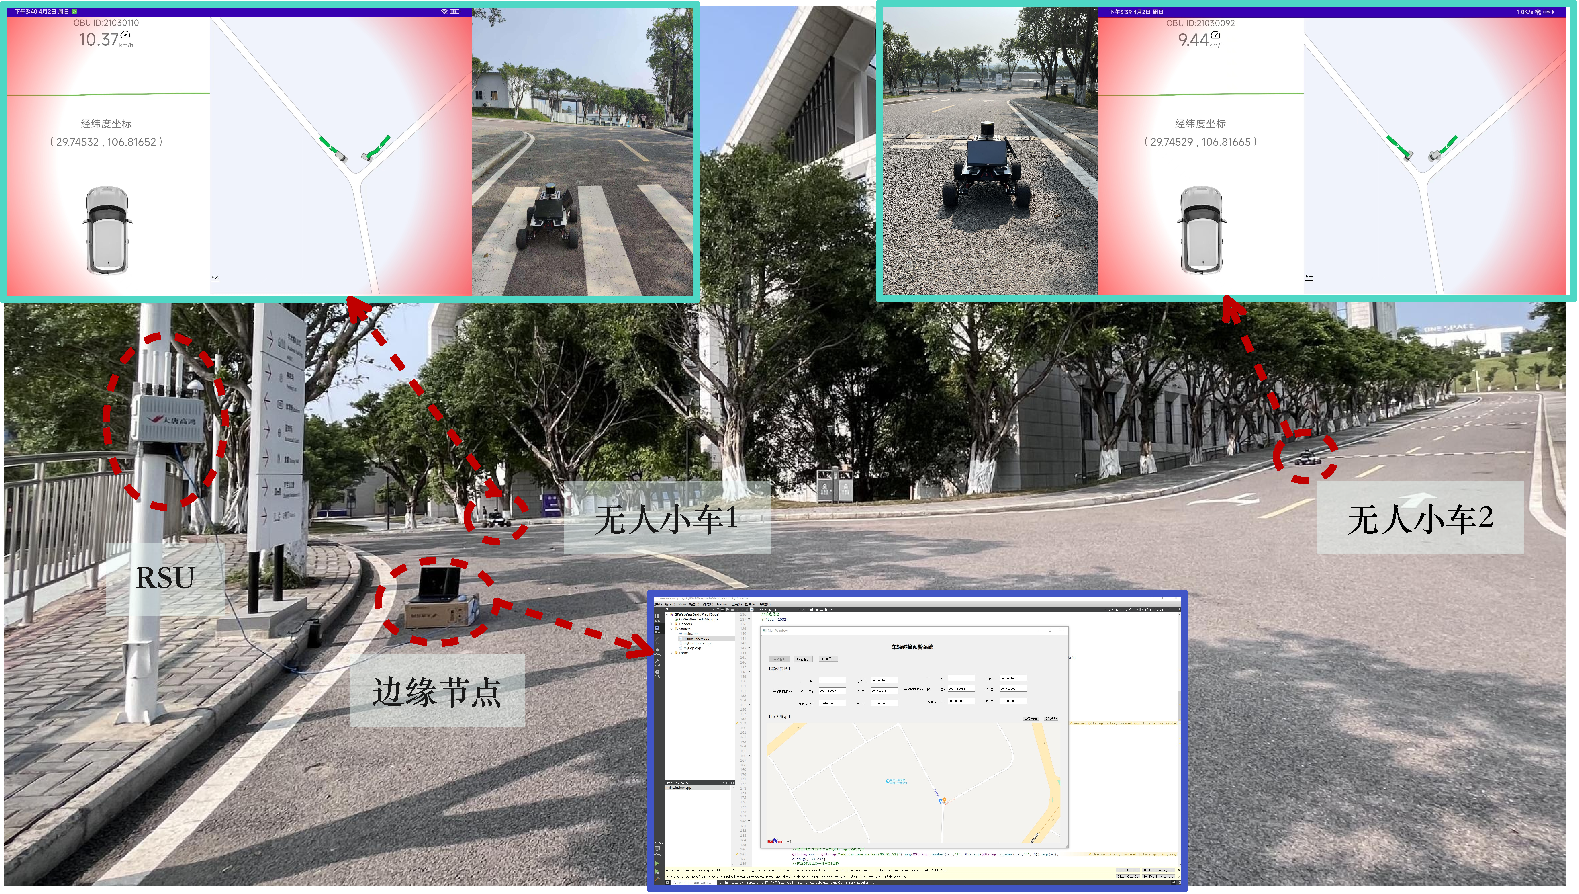
\includegraphics[width=1\columnwidth]{Fig5-12-outdoor.pdf}
  \bicaption[基于无人小车的超视距碰撞预警原型系统]{基于无人小车的超视距碰撞预警原型系统}[Non-light-of-sight collision warning prototype system based on unmanned vehicles]{Non-light-of-sight collision warning prototype system based on unmanned vehicles}
  \label{fig 5-11}
\end{figure}


\begin{figure}[h] 
	\centering
	\includegraphics[width=1\columnwidth]{Fig5-12.pdf}
	\bicaption[基于真实车辆的超视距碰撞预警原型系统]{基于真实车辆的超视距碰撞预警原型系统}[Non-light-of-sight collision warning prototype system based on real vehicles]{Non-light-of-sight collision warning prototype system based on real vehicles}
	\label{fig 5-12}
\end{figure}

本章节基于无人小车搭建验证平台如图 \ref{fig 5-11} 所示,具体地,无人小车搭载了OBU,可以通过V2I通信将自身车辆状态信息上传至位于路侧的边缘节点。
无人小车上配备NVIDIA Jetson AGX Xavier边缘计算单元,运行Ubuntu 18.04 操作系统,并配备包括激光雷达、双目视觉传感器等传感器设备。
进一步,本章分别在基于安卓系统的平板电脑和基于Qt5 平台的笔记本电脑上开发了车端应用以及边缘设备软件,其中部署了基于视图修正的碰撞预警算法,并在真实复杂车联网环境中实现了超视距碰撞预警原型系统如图 \ref{fig 5-12} 所示。
在三叉路口的基础设施上部署了RSU,其与笔记本电脑通过网线相连并被视为边缘节点。
边缘节点接收无人小车上传的状态信息并进行通过基于视图修正的碰撞预警算法进行评估是否存在潜在碰撞风险,如果存在,则通过V2I 通信将碰撞预警消息发送至无人小车并在车机界面中展示。
图 \ref{fig 5-12} 中左上和右上角分别显示了无人小车1和无人小车2的自身视角以及车机界面展示。
可以看到,无人小车分别位于三叉路口中的两条支路上,由于地势的差异(无人小车1位于上坡路段,无人小车2位于下坡路段),两车在当前位置无法通过基于视距的传感设备感知到彼此,因而具有潜在碰撞风险。
当两辆车辆分别驶向路口时,边缘节点通过V2I通信接收车辆信息,并基于所提算法判断当前存在碰撞风险,因此,无人小车接收到预警信息并在车机界面通过红色边框效果进行展示。

碰撞预警服务旨在在两车之间有可能发生碰撞时触发警告信息,从而提高车辆的安全性。
在本系统中,云服务器配备2.5 GHz的CPU和2G的内存,而SDN控制器则可以通过基于LTE的通信与车辆进行通信。
为了支持大规模和实时的碰撞预警服务,计算和通信的工作量被卸载到实现服务功能的边缘服务器上。
如图\ref{fig 5-12}所示,本章考虑的场景是在道路交叉口部署一个RSU,一台笔记本与RSU连接,作为边缘服务器,并配备1.6GHz CPU和8G内存。
在该场景中,两辆汽车(即V1和V2)正在向十字路口移动,并相互靠近。
每辆车都配备了一个OBU,其与一个基于Android的平板电脑相连。
本章开发了一个基于Android系统的应用程序,用于收集车辆的实时状态,包括GPS坐标、速度、加速度、方向和时间戳等。
对于基于边缘的服务,车辆通过 DSRC 通信向边缘节点更新其状态。
根据从不同车辆收到的信息,边缘节点执行碰撞检测服务程序。
一旦检测有碰撞的风险,预警信息就会被触发,并通过 I2V 通信传送给相应的车辆。
然后,车辆中搭载的平板电脑上会显示一个停车标志,并伴随着振动和警告音。

\section{本章小结}\label{section 5-6}

本章首先提出了一个基于逻辑视图的超视距碰撞预警场景,以支持安全关键的ITS应用。
在此场景中,车辆周期性上传自身状态信息,边缘节点基于车辆信息构建逻辑视图以反映车辆实时状态,并在此基础上,为车辆提供碰撞预警服务。
其次,本章提出了一种基于视图修正的碰撞预警算法,该算法通过结合传输延迟估计和数据包丢失检测来校准视图,使得边缘节点能够构建更加实时准确的视图。
具体地,通过推导一个基于稳定分布的应用层数据包传输延迟拟合模型来估计传输延迟,其中的拟合数据是通过现场测试获得。
另一方面,根据历史信息,包括数据传输频率和车辆的位置,检测数据包丢失。
再次,建立了基于真实车辆轨迹的仿真模型,仿真结果表明所提VCCW算法与基于云和基于边缘的碰撞预警算法相比,在碰撞预警的查准率和查全率方面都有优势。
最后,本章搭建了基于C-V2X的硬件在环试验平台,对C-V2X端到端传输性能进行了分析。进一步,搭建了基于无人小车的验证平台,其中部署了基于视图修正的碰撞预警算法,并在真实复杂车联网环境中实现了超视距碰撞预警原型系统,验证了所提系统的有效性。